\chapter{Increment three}
\label{chap:Increment three}
The procedure of this increment will be the same as the previous ones. The requirements from section \ref{sec:i2Evaluation} in increment two, will be the base for this increment. The requirements in focus will be discussed, tried implemented and the evaluated upon, which might lead to changes of the requirements list. 

\section{Requirements}
\label{sec:i3Requirements}

\begin{itemize}
	\item The trash bin should catch the trash if the user throws it towards the trash bin and within a predefined area
	\begin{itemize}
		\item {The robots predefined area should be calculated from the hardware limitations of the motors’ speed}
	\end{itemize}
	\item The robot should know where it is positioned
	\begin{itemize}
		\item {The robot should have a starting position, from where it should be able to calculate it's current position through calculations of the motor encoders}
		\item {The robot's starting point should be placed outside its predefined area, such that it moves forward into the area}
	\end{itemize}
	\item The robot should be able to detect and track the thrown trash
	\begin{itemize}
		\item {The thrown trash should be detected and tracked by a Microsoft Kinect}
		\item {The Kinect should send the coordinates of the impact point of the trash to the robot}
	\end{itemize}
	\item The robot should know where the the thrown trash will land
	\begin{itemize}
		\item {Trajectory prediction should be used to calculate impact point of the thrown trash}
	\end{itemize}
	\item The robot should be able to move the trash bin, such that the thrown trash lands inside the bin
	\begin{itemize}
		\item {The robot should be able to turn and drive forward}
		\item\textcolor{blue}{The robot should be able to recognize the coordinates sent from the Kinect}
	\end{itemize}
	\item {The robot should be able to receive data from a computer, through a wireless network}
	\item \textcolor{blue}{The system tasks should be able to be scheduled and verified}
\end{itemize}

\section{System design}
\label{sec:i3System design}
This section will describe and explain the marked requirements, for how they are planned to be fulfilled.

\subsection{Connecting Arduino and Kinect}
\label{sec:i3Connecting Arduino and Kinect system design}
For connecting the Arduino and Kinect, the Wifi library is used as explained in Appendix \ref{sec:Connecting Arduino and Kinect}. The Kinect should create a TCP-client, which should send the appropriate data to the Arduino. This TCP-client should connect when it can send data, and disconnect after sending the data, since the Arduino has a timer that closes the connection after 10 seconds of inactivity. The sent data should be of the form (x, z) expressing the distance from the kinect to the impact point of the object and the ground. The x-coordinate should express the horizontal position, and the z-coodinate should express the depth position. As the Kinect camera should be position and tilted so that the bottom angle of the cameras point of view is parallel to the ground, makes the y coordinate useless, as the impact point would always be at (x, (y = 0), z). This delimitation also gives the camera a sense of where the ground is, since it would not be able to see the ground, and therefore would calculate a different impact point, as the object would in a sense fall through the ground in the picture. 

\subsection{Scheduling}
\label{sec:i3Scheduling}
To be able to schedule the systems functions(also called tasks), the worst-case execution time(WCET) have to be known for the individual functions. The first attempt was to count the clock cycles in the assembly file of the complied arduino code. It was known that the Arduino mega 2560 has 16000 clock cycles per millisecond, so it will be possible to calculate the time for the functions. The purpose was to count the clock cycles for the two functions driveTowardsGoal and updatePosAndHead, to make that a possibility many of the functions in the different libraries used also had to be counted, the results of this can be found in Appendix \ref{chap:Clock cycles}.

In the following list, the clock cycles counted of the two functions are shown:
\begin{itemize}
	\item driveTowardsGoal = \textbf{4185} + (13)* + (174 + (13)*)* + (231 + (13)*)* + (17)* + (8)* + (33 + (17)*)* + (7)* + (5)* + (290 + (5)*)*
	\item updatePosAndHead = \textbf{3560} + (11)* + (13)* + (7)* + (174 + (13)*)* + (231 + (13)*)* (10)* + (24)* + (17)* + (33 + (17)*)*
\end{itemize}
The bold number is the worst-case of clock cycles counted in the function. The numbers in parentheses are loops, which bound is unknown, therefore it is not possible to make a count the exact WCET by counting the clock cycles.

Since it was not possible to count the clock cycles from the assembly code, it was decided to use the tool Bound-T, which will calculate the WCET outputted with an output in clock cycles. \newline
Bound-T was not able to calculate the WCET for the code. When Bound-T gets to calculating the floats, it is failing. It can't set an upper bound for the floating point numbers' WCET.

To be able to work around the float issues with Bound-T, a library called AVRFIX made by Maximilian Rosenblattl and Andreas Wolf \citep{AVRFIX}. In the listings \ref{Update1} and \ref{Update2} a function written with the AVRFIX library and a function written normally for arduino can be compared. Be aware that the function in listing \ref{Update2} might not look exactly like this in the final code for the project. 

\begin{lstlisting}[caption={The function updatePosAndHead with AWRFIX library}, label={Update1}]
void updatePosAndHead(){
int currentLeft = leftTotal;
int currentRight = rightTotal;
fix_t distPrDeg = ftok(DISTPRDEGREE);
fix_t dltL = itok(currentLeft - leftTemp);
fix_t dltR = itok(currentRight - rightTemp);
fix_t deltaLeft = mulk(dltL, distPrDeg);
fix_t deltaRight = mulk(dltR, distPrDeg);
leftTemp = currentLeft;
rightTemp = currentRight;
fix_t deltaSum = deltaLeft + deltaRight;
fix_t dist = divk(deltaSum,ftok(2.0));
fix_t sinHeading = sink(heading);
posX += mulk(dist, sinHeading);
fix_t cosHeading = cosk(heading);
posY += mulk(dist, cosHeading);
fix_t rel = divk((deltaRight - deltaLeft),ftok(WHEELDIST));
heading += atank(rel);
}
\end{lstlisting}

\begin{lstlisting}[caption={The function updatePosAndHead from the Arduino IDE}, label={Update2}]
void updatePosAndHead(){
int currentLeft = leftTotal;
int currentRight = rightTotal;
double deltaLeft = (currentLeft - leftTemp) * DISTPRDEGREE;
double deltaRight = (currentRight - rightTemp) * DISTPRDEGREE;
leftTemp = currentLeft;
rightTemp = currentRight;
double dist = (deltaLeft + deltaRight) / 2.0;
posX += (dist * sin(heading));
posY += (dist * cos(heading));
heading += (atan((deltaRight - deltaLeft) / WHEELDIST));
}
\end{lstlisting}

The program was rewritten with the AVRFIX library and then using Bound-T again to calculate the worst-case execution time for the functions. The AVRFIX library came with a .txt file from the GitHub download, which included the clock cycles for the AVRFIX functions. \newline
The function updatePosAndHead is calculated to use 3995 clock cycles, but when trying to calculate the function driveTowardsGoal another problem occurred. When a division by 0 took place, the program will enter an infinite loop, making it impossible to set an upper bound on the WCET. With this problem it is not possible to calculate the WCET for driveTowardsPoint.

Because using the AVRFIX library with Bound-T also failed, the group decided to use the function micros() on the functions to measure the time spent on the function, run them several times and use highest result as WCET. 

The WCET for the two functions using the Micros() function, is listed below:
\begin{itemize}
	\item updatePosAndHead = 1076 microseconds
	\item driveTowardsGoal = 732 microseconds
\end{itemize}

The above results will be used for a schedulability analysis made in UPPAAL in section \ref{sec:i3UPPALL model}. 
\section{Implementation}
\label{sec:i3Implementation}
This section will describe if the requirements were fulfilled through implementation.

\subsection{Connecting Arduino and Kinect}
\label{sec:i3Connecting Arduino and Kinect implementation}

\subsection{UPPAAL model of schedulability}
\label{sec:i3UPPAAL model}
To create the UPPAAL model and to check the schedulability of the tasks used for Dumpsty, every tasks WCET is calculated. This execution time is attained through running the code multiple times with a set timer, and writing the timer in a log after executing the specific task. There are three tasks for Dumpsty: Updating the position and heading (referred to as "PrA"), driving towards the goal position ("PrB") and the WiFi code that has to be looped ("PrC"). Here are the WCET attained through the tests, and to the right of the clock cycles is the WCET used in UPPAAL. The WCET used in UPPAAL has a significant margin greater than the WCET gained through the tests, since there is enough time to give each task a greater WCET, and the worst case tested is not necessarily the WCET of the tasks. 

\begin{itemize}
	\item PrA \tab Tested: 1067 microseconds \tab UPPAAL: 2 milliseconds
	\item PrB \tab Tested: 732  microseconds \tab UPPAAL: 1 milliseconds
	\item PrC \tab	Tested: 8469 microseconds \tab UPPAAL: 9 milliseconds
\end{itemize}

The interrupt generated by the motor encoders is taken into account in every task, but to simplify the schedulability analysis, the WCET of the interrupt has been multiplied to the WCET of every greater task. Therefore the interrupt and the interrupt handler is not considered as a task, but as a part of the other tasks.

When describing these tasks in UPPAAL, two different classes were declared: One to instantiate a cyclic executive task instance of every task, and a CPU class to control the synchronization between all the tasks, as shown in the following figure:

\begin{figure}[h]
	\centering
	\fbox{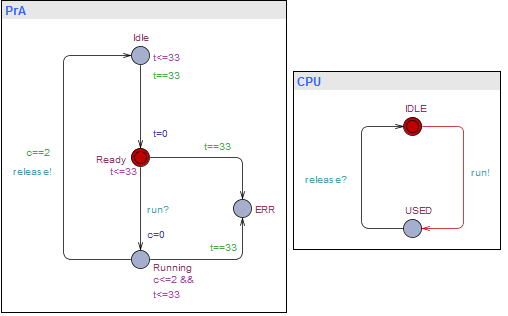
\includegraphics[scale=0.60]{billeder/UPPAALPr}}
	\caption{Automata in UPPAAL}
	\label{robot}
\end{figure}

When the automata of the tasks has been created, every task has to be declared with an ID, a deadline and a period. The deadline has been declared for every task to be within the MIT of coordinates from the Kinect sensor, which is 33 milliseconds.
The tasks are declared as:

\begin{itemize}
	\item PrA = TASK(1, 33, 2);
	\item PrB = TASK(2, 33, 1);
	\item PrC = TASK(3, 33, 9);
\end{itemize}

After creating the automata and declaring the tasks, the UPPAAL schedulability analysis can be done. This is done through the verifier in UPPAAL, with two different queries:

\begin{lstlisting}[caption={Queries for UPPAAL}, label={Queries}]
	E<> PrA.Ready and PrB.Ready and PrC.Ready and PrA.t==0 and PrB.t==0 and PrC.t==0 and time>0
	E[] not (PrA.ERR or PrB.ERR or PrC.ERR)
\end{lstlisting}

The first query dictates that each tasks instance should be in a ready state, each tasks should have completed within the deadline and some interval of time has to be passed. This creates a scenario where the tasks has all been executed, and none of them have exceeded the deadline.
The second query dictates that no task should ever enter an error state.
After verifying both queries it is possible to say whether the tasks can be scheduled or not, in this case it is possible.

\section{Evaluation}
\label{sec:i3Evaluation}
Many different methods were used to try to calculate the WCET for the systems functions. At first it was tried to count the clock cycles from the complied assembly code, which proved to be very difficult, since the bounds of the libraries was unknown. Because of these problems third party software and libraries was used to calculate the WCET, but the once again without any success. The method used to calculate the WCET was to use the micros() function, available in the arduino IDE, to measure the time used on the function, which would give close to a WCET of the functions. The tasks all had a significant margin to improve the possibility of hitting actual WCET. \newline
The WCET's were used with the software UPPALL, as described in section \ref{sec:i3UPPAAL model}. This concluded that the tasks was easily schedulable within the defined deadlines.

